\documentclass{article}
\usepackage{package}
\graphicspath{ {./images/} }

\makeindex


\title{
    {\LARGE ASCON v1.2}\\
    \vskip 0.1cm{\Large Analisi e implementazione}
    %\vskip 0.8 cm{\Large Facolt\`a di Scienze e Tecnologie}\\
    \vskip 0.4cm{\large CdL in Sicurezza dei Sistemi e delle Reti Informatiche}
}
\author{
    \Large Melissa Moioli, Mattia Perfumo, Tiziano Radicchi\\
    \large 09831A, xxx, 12172A
}
\date{
    {\large\today}
}

\makeatletter
\newcommand{\@alphalph}{}% Check that \@alphalph is undefined.
\let\@alphalph=\alphalph
\makeatother


\begin{document}
\pagenumbering{gobble}

\begin{titlepage}
    \pagestyle{empty}
    %\selectlanguage{italian}
    \maketitle
    %\selectlanguage{english}
    \vspace{2em}
    \begin{abstract}
        \textit{\noindent
Si propone un'analisi della famiglia di schemi di cifratura autenticata e hashing ASCON, selezionata come soluzione primaria per la realizzazione di lightweight cryptography nella competizione CAESAR nonché come famiglia adatta a standardizzazione NIST. Si propone in aggiunta una implementazione di ASCON-128 e ASCON-HASH, nonché una dimostrazione di utilizzo del cifrario in sistemi embedded.  }
        %\textit{\kant[1]}% TODO 
    \end{abstract}
    \vskip 4cm\centerline{
\includegraphics[height=50mm]{./src/unimi}}
    \newpage
    \pagenumbering{Roman}
    \tableofcontents
    %\selectlanguage{italian}
    \vspace{\fill}
\end{titlepage}

\pagenumbering{arabic}
\lhead{
    ASCON - Analisi e implementazione
}
\rhead{Moioli, Perfumo, Radicchi}

\section{Introduzione}
Con questo documento intendiamo proporre un'analisi e implementazione dello schema di cifratura \textbf{ASCON-128}, facente parte di una famiglia più ampia di cifrari e algoritmi di hashing. In particolare, sono presenti: 
\begin{itemize}
    \item \textsl{ASCON-128a}: Cifrario a blocchi di 128 bit anziché 64
    \item \textsl{ASCON-80pq}: maggiore robustezza contro ricerca della chiave tramite quantum-computing (chiave da 160 bit)
    \item \textsl{ASCON-HASHa}
    \item \textsl{ASCON-XOF}: Extendable output function per produrre hash outputs di lunghezza arbitraria
    \item \textsl{ASCON-XOFa}
\end{itemize}
Tutti gli schemi forniscono una sicurezza di 128-bit ed utilizzano una matrice di stato da 320-bit nei processi di cifratura, decifratura ed hashing. Le raccomandazioni NIST includono le combinazioni ASCON-128 + ASCON-HASH oppure ASCON-128a + ASCON-HASHa.
\subsection{Agenda}
Nelle sezioni successive si introdurrà in maniera più dettagliata il funzionamento ed i parametri per l'utilizzo del cifrario; si analizzeranno le strutture scelte, effettuando richiami e confronti (ove possibile) con gli argomenti affrontati durante l'insegnamento di \textsl{Crittografia}. Si proseguirà poi con una implementazione in linguaggio C del cifrario, con delle dimostrazioni di utilizzo, per concludere infine con una proposta di applicazione dello schema in uno scenario di comunicazione wireless tra sistemi embedded, al fine di ricreare uno scenario realistico e dimostrare l'utilizzabilità dello schema in ambienti con potenza di calcolo, memoria e energia limitate. 

\newpage
\section{Specifica}
\subsection{Introduzione}
La suite ASCON fornisce la cosiddetta \textbf{Authenticated Encryption with Associated Data (AEAD)}, nonché le funzionalità di hashing già citate.
\newline
Un cifrario autenticato consiste in uno schema di cifratura che possa assicurare, oltre alla più ovvia confidenzialità dei dati cifrari, l'integrità di questi, affinché il ricevente possa assicurarsi che il messaggio durante il transito non abbia subito distorsioni, dovute a disturbi o più importante a tampering da parte di un'entità terza. ASCON assicura l'integrità del messaggio trasmesso, nonché di eventuali dati associati. L'idea alla base è quella di restituire, al termine della cifratura, un \textbf{tag} da 128 bit estratto dallo state alla fine della procedura di cifratura. Lo state utilizzato per la cifratura, con riferimento ai diagrammi più avanti riportati, dipende anche da eventuali dati associati. In questo modo si può assicurare l'inegrità anche di quei metadati per i quali non è necessaria la confidenzialità, ma per i quali ci si vuole comunque assicurare dell'assenza di manipolazioni da parte di threat actors.
\newline\newline
Tutti gli schemi si basano su una funzione $p$, composta da somme, sostituzioni e permutazioni (più avanti approfondite) e che opera su una matrice di stato da 320 bit. La funzione è stata ideata per assicurare robustezza a fronte delle limitazioni hardware e software che un sistema embedded può imporre. Le operazioni sono \textbf{definite su parole da 64 bit} e trattandosi di \textbf{operazioni logiche} (AND, NOT, XOR, ROT), l'implementazione dello schema risulta particolarmente ottimale per ambienti di questo tipo. Inoltre, si adatta particolarmente a scenari in cui dispositivi trasmettono poche informazioni in maniera periodica: dai benchmark risulta che lo schema è particolarmente efficiente per messaggi brevi.
\newline\newline
Non vi è necessità di operazioni inverse, dal momento in cui $p^a$ e $p^b$ sono valutati in una sola diretazione sia per cifratura che decifratura. 
\newline\newline
ASCON non utilizza key scheduling o espansione di chiave. Non ci sono costi aggiuntivi quando la chiave viene cambiata. 
\subsubsection{Authenticated Encryption}
Per realizzare la cifratura con autenticazione dei dati gli algoritmi in ASCON sono parametrizzati tramite:
\begin{itemize}
    \item Lunghezza della chiave $k < 160$ bits
    \item Rate (dimensione del blocco) $r$
    \item Numero di round interni $a$ e $b$
\end{itemize}
Così facendo ogni schema definisce la propria funzione di cifratura $\epsilon_{k, r, a, b}$ e decifratura $D_{k, r, a, b}$. La procedura di cifratura prende in input una chiave $K$, un \textsl{nonce} $N$ da 128 bit, eventuali dati associati $A$ ed un plaintext $P$ di lunghezza arbitraria. Restituisce un ciphertext $C$ della medesima lunghezza del plaintext. Dunque
\[\epsilon_{k,r,a,b}(K,N,A,P)=(C,T)\]
La procedura di decifratura restituisce un plaintext se e solo se l'integrità è assicurata, ovvero previa uguaglianza del tag ricevuto e del tag ricacolato
\[D_{k,r,a,b}(K,N,A,C,T)\in\{P, \bot\}\]
\subsubsection{Hashing}
TODO

\subsubsection{Parametri}
Per quanto riguarda i parametri suggeriti:
\begin{table}[h!]
    \centering
    \begin{tabular}{|c|c|c|c|c|c|c|c|}
        \hline
        \textbf{Nome}       & \textbf{Algoritmo}            & \textbf{k} & \textbf{nonce} & \textbf{tag} & \textbf{blocco} & \textbf{a} & \textbf{b} \\
        \hline
        \textsl{ASCON-128}  & $\epsilon, D_{128, 64,12,6}$  & 128        & 128            & 128          & 64              & 12         & 6          \\
        \hline
        \textsl{ASCON-128a} & $\epsilon, D_{128, 128,12,6}$ & 128        & 128            & 128          & 128             & 12         & 8          \\
        \hline
    \end{tabular}
\end{table}

\subsubsection{State}
Tutti i design della suite utilizzato uno state da 320 bit, gestito tramite 5 parole da 64. Lo state viene aggiornato con la funzione $p$, ripetuta $a$ o $b$ volte in base alla fase in cui ci si trova (inizializzazione, cifratura/decifratura, finalizzazione). 

\subsection{Authenticated Encryption}
La modalità utilizzata da ASCON è basata sulle modalità \textbf{duplex} come \textsl{MonkeyDuplex} e \textsl{Sponge-based} design, seppur utilizzi una \textbf{inizializzazione} e \textbf{finalizzazione} (entrambe basate su chiave) più robuste. L'operazione di cifratura e decifratura avviene come in figura: 
\begin{figure}[h!]
    \centering
    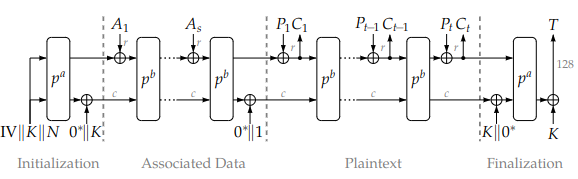
\includegraphics[width=12cm]{images/enc.png}
    \caption[short]{$\epsilon_{k,r,a,b}$}
\end{figure}
\begin{figure}[h!]
    \centering
    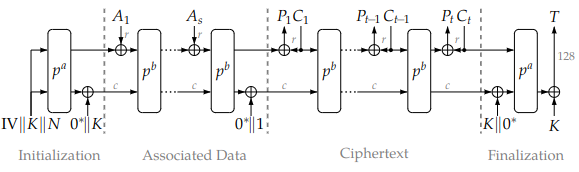
\includegraphics[width=12cm]{images/dec.png}
    \caption[short]{$D_{k,r,a,b}$}
\end{figure}
\paragraph*{Inizializzazione}
L'inizializzazione prevede uno state di partenza con la seguente forma: 
\[S \leftarrow IV_{k,r,a,b} || K || N\]
\[IV_{k,r,a,b} \leftarrow k || r || a || b || 0^{160-k} = 80400c0600000000\;\;\;\;per\;ASCON-128\]
L'inizializzazione si conclude con:
\[S\leftarrow p^a(S)\oplus (0^{320-k} || K)\]
\paragraph*{Dati associati}
I dati associati sono processati in blocci da $r$ bit. L'eventuale padding viene realizzando con l'append di un 1 finale ed il minor numero di 0 necessari per raggiungere una lunghezza che sia multiplo di $r$. Nel caso in cui non ci dovessero essere dati associati, si passa direttamente alla fase di cifratura/decifratura. Ogni blocco di dato associato viene messo in XOR con i bit più significativi dello state e la porzione di state sostituita con il risultato. Questo implica che il tag finale dipenderà anche dal valore dei dati associati e la verifica fallirà a fronte di un tampering di questi. 
\newline\newline
Alla fine di questa fase, lo state viene messo in XOR con 1 come costante di separazione del dominio. Questa operazione è svolta come contromisura di alcuni attacchi che potrebbero cambiare il ruolo dei blocchi di plaintext e dati associati. 
\paragraph*{Cifratura/Decifratura}
Come per i dati associati il plaintext/ciphertext viene suddiviso in blocchi con eventuale 1 + padding. Durante la cifratura, ad ogni XOR lo state viene aggiornato con il risultato dell'operazione. L'ultimo blocco di ciphertext viene troncato alla lunghezza dell'ultimo blocco di plaintext senza padding, in modo tale da preservare la lunghezza originale del messaggio. Si riapplica $p^b$ dopo ogni XOR ad eccezione dell'ultimo. 
\newline\newline
Per la decifratura invece il blocco di ciphertext viene inserito nello state ed utilizzato per effettuare uno XOR, in modo da recuperare il plaintext originale. Si riapplica $p^b$ dopo ogni XOR ad eccezione dell'ultimo. 
\newline\newline
Si noti come in assenza di dati associati e in presenza di un singolo blocco di plaintext da cifrare, non sono necessarie altre $p^b$ sullo state. Per prevenire lo scenario in cui lo XOR della chiave si cancelli, lo XOR viene effettuato su due parti dello state diverse. 
\paragraph*{Finalizzazione}
Durante la finalizzazione la chiave $K$ viene XORata con lo state, per poi applicare $p^a$. Si estrae dunque il tag $T$ dai 128 bit meno significativi dello state XORati con la chiave $K$. 
\subsection{Funzione $p$}
La funzione $p$ introduce le proprietà di confusione, tramite S-Box, e diffusione, tramite il linear layer. Ogni round $p$ è un SPN-based round.  
\begin{figure}[h!]
    \centering
    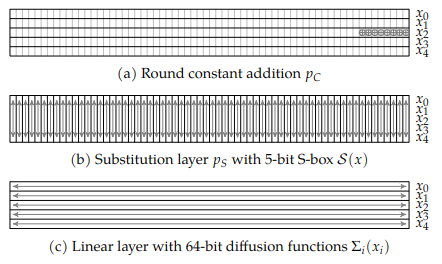
\includegraphics[width=10cm]{images/p.png}
\end{figure}
\begin{figure}[h!]
    \centering
    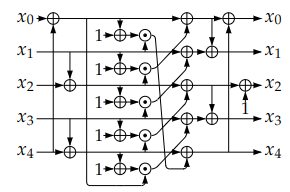
\includegraphics[width=6cm]{images/sbox.png}
    \caption[short]{Approccio bitsliced per applicazione della S-Box}
\end{figure}
\newline
La prima operazione svolta è uno XOR con una costante. La costante è identificata dal numero di round in cui ci si trova. Si passa poi alla sostituzione tramite S-Box, la cui implementazione è preferibile nella sua forma \textsl{bitsliced} con operazioni effettuate sulle intere parole da 64 bit. Infine si passa al layer di diffusion, dove ad ogni parola da 64 bit si applicano degli XOR con la medesima parola ruotata di un determinato numero di bit a destra. 
\paragraph*{Costante di round}
Le costanti di round sono state scelte grandi abbastanza per evitare \textsl{slide, rotational, sel-fimilarity} o attacchi simili. La scelta è stata effettuata in maniera semplice, ovvero incrementando o meno un counter. La posizione invece è stata scelta per permettere il pipelining con le operazioni precedenti e successive (ad esempio le istruzioni successive per le S-box). 
\paragraph*{Sobstitution layer}
Il layer di sostituzione è l'unica porzione non lineare del round. Mixa i 5 bit che compongono una colonna nello state.

\subsection{ASCON-128}
Si tratta di un cifrario a blocchi che prevede operazioni di sostituzione e permutazione, nonché di somma e rotazioni di bit. Come accennato tutte le operazioni sono ripetute in più round ed implementate unicamente tramite bitwise operations.

\newpage
\section{Design Rationale}
La suite è basata sullo \textbf{sponge design}. La funzione $p$ è basata su SPN (Substitution-Permutation-Network). Per questo le componenti principali del cifrario sono ispirate a schemi già standardizzati. 
\newline\newline
Il substitution layer utilizza una sostituzione affine equivalente alla S-Box utilizzata in \textsl{SHA-3}. Il permutation layer utilizza funzioni lineare simili a quelle utilizzate da SHA-2. 
\newline\newline
Lo sponge-based design in particolare si avvicina allo \textsl{SpongeWrap} e al \textsl{MonkeyDuplex}. Lo sponge-based design ha diversi vantaggi rispetto ad altre tecniche di costruzione come i tradizionali cifrari a blocchi o le modalità hash-based: 
\begin{itemize}
    \item Ampiamente studiate ad analizzate con diverse dimostrazioni sulla solo sicurezza. Utilizzate in SHA-3
    \item Design semplice, privo di key scheduling
    \item I blocchi di plaintext e ciphertext possono essere computati direttamente, senza attendere per la ricezione del messaggio completo o di conoscere la lunghezza di esso. 
    \item Utilizzo della medesima funzione sia per cifrare che per decifrare. 
\end{itemize} 
\subsection{Sponge Function}
TODO
\subsection{MonkeyDuplex}
TODO
\newpage
\section{Crittoanalisi}
\subsection{Security Claims}
Tutti i design della suite offrono una sicurezza a 128 bit. Il numero di blocchi di plaintext e dati associati processati e protetti dallo schema è limitato a $2^{64}$ blocchi per chiave, che corrispondono a $2^{67}$ bytes (per ASCON-128). Al fine di assicurare una sicurezza a 128 bit le implementazioni devono assicurarsi che il nonce non sia ripetuto per più di due cifratura con la stessa chiave. 
\newline\newline
Inoltre il design assicura sicurezza anche di fronte ad alcuni errori implementativi, come i nonce ripetuti. Ulteriormente, anche un recupero completo di uno state durante l'elaborazione dei dati associati, del plaintext o del ciphertext non implica la possibilità di effettuare attacchi di recupero della chiave. 
\newline\newline
Non vi sono ulteriori limitazioni sulla scelta del nonce, che può essere scelto anche in maniera incrementale. Come per il resto dei cifrari, anche nel caso di ASCON osservano il ciphertext si può scoprire la lunghezza del plaintext, a meno ulteriori padding extra alla specifica. 
\newline\newline
Durante i test crittoanalitici nella competizione CAESAR tutte le analisi hanno restituito un buon margine di sicurezza, senza alcuna indicazione relativa a possibili debolezze. I miglior attacchi si sono incentrati su implementazioni con un numero di round ridotto nella fase di inizializzazione dello schema da 12 a 7 round, mantenendo comunque l'attacco lontano dall'essere una minaccia effettiva. 
\newline\newline
Lo schema è stato disegnato per assicurare una robustezza di fronte ad eventuali errori implementativi. Ad esempio, se un attacco dovesse essere in grado di recuperare uno state interno durante il processamento dei dati (ad esempio tramite un attacco side-channel), questo non permetterebbe comunque di recuperare direttamente la chiave. 
\newline\newline
Particolare attenzione all'implementazione delle S-Box: la possibilità di definire le sostituzioni realizzate tramite S-Box direttamente attraverso operazioni bitwise sullo state rendono evitabile un'operazione di table lookup. Una tale operazione risulterebbe infatti onerosa di risorse computazionali e aprirebbe le porte ad eventuali side-channel attack, dal momento in cui sarebbe possibile identificare l'istante temporale in cui il lookup avviene osservando la variazione di consumo energetico del sistema. La protezione da side-channel attack rappresenta di uno degli obiettivi principali di ASCON. A questo scopo è importante che sia semplice proteggere la S-Box. La sua implementazione permette proprio di contrastare questi attacchi. 
\subsection{Security Analysis}
Seguono i report di diversi attacchi noti testati sullo schema di cifratura. Le permutazioni di ASCON non sono considerate come delle permutazioni ideali di 320 bit, ma con i parametri suggeriti permettono comunque di ottenere un generoso margine di sicurezza. 
\newline\newline
Attualmente, il miglior attacco crittoanalitico può recuperare la chiave con una complessità in tempo di $2^{104}$ se e soltanto se l'inizializzazione è ridotta a 7 round. 
\subsubsection{Crittoanalisi differenziale e lineare}
Di seguito in figura DDT (Differential Distribution Table) e LAT (Linear Approximation Table). 
\begin{figure}[h!]
    \centering
    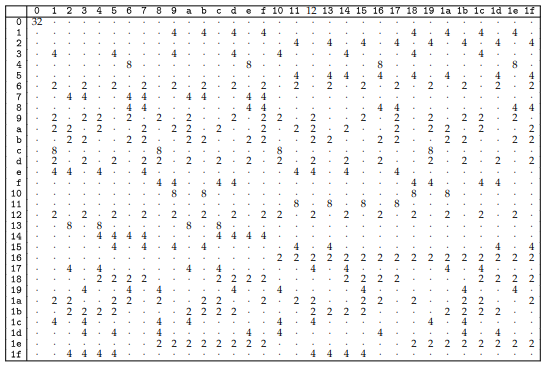
\includegraphics[width=12cm]{images/ddt.png}
    \caption[short]{DDT}
\end{figure}
\begin{figure}[h!]
    \centering
    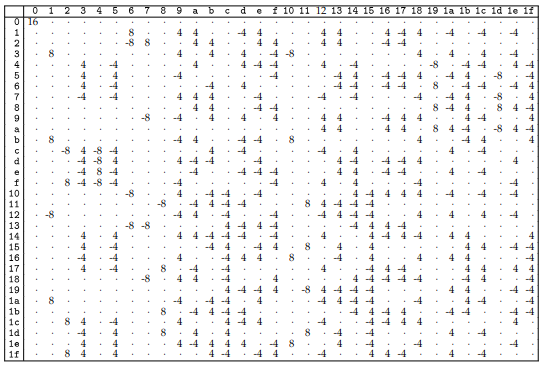
\includegraphics[width=12cm]{images/lat.png}
    \caption[short]{LAT}
\end{figure}

\newpage
\section{Protocollo di comunicazione}
Si passa ora alla proposta di implementazione di un semplice protocollo di comunicazione half-duplex che fa uso dello schema appena implementato. 
\newline\newline
In particolare, si propone un protocollo di comunicazione tra due dispositivi embedded, uno dei quali funge da \textsl{master} e l'altro da \textsl{slave}. Il protocollo da cui si è stati ispirati corrisponde ad uno \textsl{Stop And Wait ARQ}: Il master invia un messaggio cifrato allo slave, che conferma la ricezione del messaggio. Il master attende la ricezione della conferma prima di trasmettere il messaggio successivo. Tecniche di controllo di errore sono implementate per rispondere ad eventuali perdite di messaggi o alterazioni del contenuto, che causerebbero un fallimento della verifica del tag. 
\newline\newline
In questa sede non si discuterà di come i due dispositivi si scambino le chiavi, ma si suppone che le chiavi siano già state scambiate in precedenza. Si suppone che entrambi i nodi, all'inizio del protocollo, condividino una chiave segreta $K$ ed un nonce $N$.
\newline\newline
Il master trasmette un messaggio con il seguente formato: 
\begin{center}
    \texttt{messageLength.\textsl{nonce....message}.tag}
\end{center}
Dove della porzione \textsl{nonce....message} ne viene trasmesso il ciphertext. 
\newline
Si trasmette la lunghezza del payload, il nonce utilizzato per la cifratura, il payload effettivo ed il tag per la verifica dell'integrità del messaggio, previsto dalla specifica di ASCON. la porzione cifrata non viene trasmessa con un particolare encoding, dunque è necessario conoscere anche la lunghezza del messaggio affinché lo schema di decifratura possa operare correttamente. Il nonce utilizzato viene utilizzato in modo tale che lo slave possa verificare che il nonce utilizzato per la decifratura corrisponda a quello utilizzato per la cifratura. Si tratta di un meccanismo ulteriore oltre al tag per verificare che la decifratura sia avvenuta in maniera corretta. In questo modo il receiver può avere la certezza di essere sincronizzato con il master circa il nonce utilizzato, per poi incrementarlo per la decifratura successiva. Infine il tag, per realizzare il processo di decifratura e verificare l'integrità. 
\newline\newline
Quando il ricevente verifica, come indicato qui sopra, la corretta decifratura del messaggio, trasmette un messaggio contente "\textsl{ok}" cifrato con il nonce concludendo con l'incremento del nonce. 
\newline\newline
Il master riceve l'ack, verifica la decifratura e se il messaggio corrisponde ad "\textsl{ok}", incrementa il nonce anche lui, per poi passare alla trasmissione successiva. 
\newline\newline
Nel caso in cui l'ack non dovesse essere ricevuto dal master, il master si occuperebbe di ritrasmettere il messaggio. Qui, due scenari: 
\begin{itemize}
    \item Il messaggio non era stato ricevuto dallo slave: entrambi sono ancora sincronizzati sul medesimo nonce, dunque ad una ritrasmissione successiva la comunicazione può riprendere
    \item Il messaggio era stato trasmesso, lo slave aveva inviato la conferma, che però non è stata ricevuta. Lo slave si trova ad un nonce successivo rispetto a quello del master. Lo slave, alla ricezione della ritrasmissione non sarà in grado di decifrare correttamente, dunque entra in uno stato di \textsl{retryNonce} in cui tenta la decifratura con il nonce precedente. Se la decifratura va a buon fine, lo slave ripristina il nonce al fine di sincronizzarsi con il master.
\end{itemize}
\subsection{Implementazione}
L'esempio implementativo proposto prevede l'utilizzo di due sistemi embedded ESP8266 e l'utilizzo di due moduli LoRa per trasmissione e ricezione. 
\newpage


\newpage
\end{document}
